\documentclass[titlepage]{article}
\usepackage[utf8]{inputenc}
\usepackage[left=1cm, top=0.8cm,bottom=1.2cm, textwidth=18.6cm, textheight=27cm]{geometry}
\geometry{paper=a4paper}
\usepackage{titling}
\usepackage{abstract}
\usepackage{fancyhdr}
\usepackage{amsmath}
\usepackage{gensymb}
\usepackage{graphicx}

\lhead{} \chead{} \rhead{}
\lfoot{\emph{Multimedia and computer visualisation 2015/2016}} \cfoot{} \rfoot{\thepage}
\renewcommand{\headrulewidth}{0pt}
\renewcommand{\footrulewidth}{0.4pt}
\pagestyle{fancy}


\title{Color systems conversion tool}
\author{Maciej Borkowski\\ 195968@student.pwr.edu.pl \and Michał Kowalski \\ 195447@student.pwr.edu.pl}
\date{}
\begin{document}
\maketitle
\section{Introduction}
%TODO

\section{Color Systems}
%TODO

\begin{itemize}
  \item RGB - red, green, blue,
  \item grayscale,
  %TODO binary,
  \item CMYK,
  \item HSV.
  %TODO YUV & YIQ
\end{itemize}

\subsection{RGB}
%TODO

\subsubsection{HEX}
Hexadecimal represetation allows to write 3 RGB values as a single value,
followed by \# sign. Conversion can be done in two ways, which give equal
results:
\begin{enumerate}
  \item $HEX=R*256^2+G*256+B$,
  \item writing RGB values as three (two-digits long, from $00$ to $FF$)
  hexadecimal numbers, and writing them next to each other.
\end{enumerate}
Second way is much easier for humans because of lower values (3 values in
range 0-255, instead of one value up to about 16M). Also reverse operation
is much easier, because it requires only splitting of a string and changing
three low values from hex to decimal, instead of many divisions and modulo
operations. Some examples of hex values are:
\begin{itemize}
  \item $(0, 0, 0) \Leftrightarrow \#000000$,
  \item $(255, 255, 255) \Leftrightarrow \#FFFFFF$,
  \item $(0, 255, 0) \Leftrightarrow \#00FF00$,
  \item $(192, 192, 192) \Leftrightarrow \#C0C0C0$.
\end{itemize}

\subsection{Grayscale}
% TODO
\subsubsection{Conversion}
Conversion from RGB to grayscale can be done by calculating average value of RGB
values, and conversion in another direction by assigning one grayscale value to
all RGB ones.

\subsection{HSV}
% TODO
\subsubsection{Conversion from RGB}
Conversion from 0-255 RGB values can be done by formula:
\begin{equation}
\begin{split}
(R', G', B')&=(R, G, B)/255\\
C_{max}&=max(R', G', B')\\
C_{min}&=min(R', G', B')\\
\Delta&=C_{max}-C_{min}\\
\\
H&=\begin{cases}
0 & \Delta=0 \\
60\degree*(\frac{G'-B'}{\Delta}mod6) & C_{max}=R' \\
60\degree*(\frac{B'-R'}{\Delta}+2) & C_{max}=G' \\
60\degree*(\frac{R'-G'}{\Delta}+4) & C_{max}=B'
\end{cases} \\
S&=\begin{cases}
0 & C_{max}=0 \\
\frac{\Delta}{C_{max}} & C_{max} \neq 0
\end{cases}\\
V&=C_{max}
\end{split}
\end{equation}

\subsubsection{Conversion to RGB}
Conversion to 0-255 RGB values can be done by formula:
\begin{equation}
\begin{split}
C&=V*S\\
X&=C*(1-|H/60\degree|mod2-1)\\
m&=V-C\\
\\
(R', G', B')&=\begin{cases}
(C, X, 0) & 0\degree\leq H < 60\degree\\
(X, C, 0) & 60\degree\leq H < 120\degree\\
(0, C, X) & 120\degree\leq H<180\degree\\
(0, X, C) & 180\degree\leq H<240\degree\\
(X, 0, C) & 240\degree\leq H<300\degree\\
(C, 0, X) & 300\degree\leq H<360\degree
\end{cases}\\
\\
(R, G, B)&=((R'+m)*255, (G'+m)*255, (B'+m)*255)
\end{split}
\end{equation}

\subsubsection{Examples}
Some examples for conversion between 0-255 RGB and HSV:
\begin{itemize}
  \item $(0, 0, 0) \Leftrightarrow (0\degree, 0\%, 0\%)$,
  \item $(255, 255, 255) \Leftrightarrow (0\degree, 0\%, 100\%)$,
  \item $(255, 0, 0) \Leftrightarrow (0\degree, 100\%, 100\%)$,
  \item $(0, 255, 255) \Leftrightarrow (180\degree, 100\%, 100\%)$,
  \item $(128, 0, 128) \Leftrightarrow (300\degree, 100\%, 50\%)$.
\end{itemize}

\subsection{CMYK}
% TODO
\subsubsection{Conversion from RGB}
Conversion from 0-255 RGB values can be done by formula:
\begin{equation}
\begin{split}
(R', G', B') &= (R, G, B)/255 \\
K&=1-max(R', G', B')\\
C&=(1-R'-K)/(1-K)\\
M&=(1-G'-K)/(1-K)\\
Y&=(1-B'-K)/(1-K)
\end{split}
\end{equation}
\subsubsection{Conversion to RGB}
Conversion to 0-255 RGB values can be done by formula:
\begin{equation}
\begin{split}
R&=255*(1-C)*(1-K)\\
G&=255*(1-M)*(1-K)\\
B&=255*(1-Y)*(1-K)
\end{split}
\end{equation}

\subsubsection{Examples}
Some examples for conversion between 0-255 RGB and CMYK:
\begin{itemize}
  \item $(0, 0, 0) \Leftrightarrow (0, 0, 0, 1)$,
  \item $(255, 255, 255) \Leftrightarrow (0, 0, 0, 0)$,
  \item $(255, 0, 0) \Leftrightarrow (0, 1, 1, 0)$,
  \item $(0, 255, 0) \Leftrightarrow (1, 0, 1, 0)$,
  \item $(0, 255, 255) \Leftrightarrow (1, 0, 0, 0)$.
\end{itemize}

\section{Application Functionality}

\begin{figure}[!htb]
	\centering
	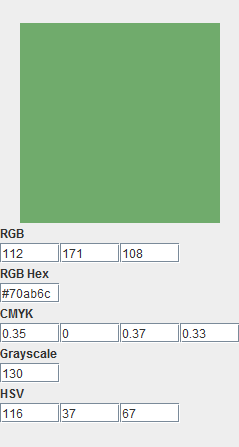
\includegraphics[width=0.35\textwidth]{img/conversion.png} 
	\caption{Color conversion panel}
\end{figure}


\begin{figure}[!htb]
	\centering
	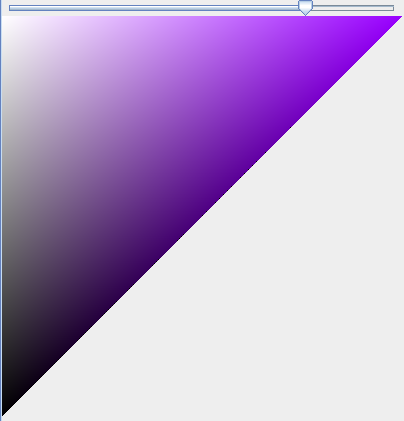
\includegraphics[width=0.5\textwidth]{img/hsvpick.png} 
	\caption{Picking color from HSV cone}
\end{figure}


\begin{figure}[!htb]
	\centering
	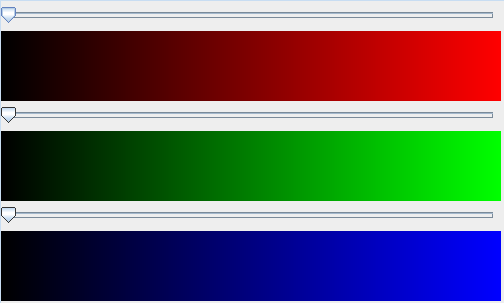
\includegraphics[width=0.7\textwidth]{img/rgbpick.png} 
	\caption{Picking color from RGB sliders}
\end{figure}


\begin{figure}[!htb]
	\centering
	
\includegraphics[width=0.4\textwidth]{img/imagepick.png}
	\caption{Picking color from image} 
\end{figure}
\end{document}